\documentclass[aps,pra,twocolumn,showpacs,superscriptaddress,floatfix,10pt]{revtex4}
\usepackage{graphicx}
\usepackage{psfrag}
\usepackage{amssymb,amsmath}
\usepackage{physics}
\usepackage{float}
\usepackage{dsfont}
\usepackage{algorithmicx}
\usepackage[noend]{algpseudocode}
%\usepackage[dvips]{color}
\algdef{SE}[DOWHILE]{Do}{doWhile}{\algorithmicdo}[1]{\algorithmicwhile\ #1}%

%\setlength{\topmargin}{0.1cm}
\begin{document}
\newcommand{\beq}{\begin{equation}}
\newcommand{\eeq}{\end{equation}}
\newcommand{\ben}{\begin{eqnarray}}
\newcommand{\een}{\end{eqnarray}}
\newcommand{\bea}{\begin{array}}
\newcommand{\eea}{\end{array}}
\newcommand{\om}{(\omega )}
\newcommand{\bef}{\begin{figure}}
\newcommand{\eef}{\end{figure}}
\newcommand{\leg}[1]{\caption{\protect\rm{\protect\footnotesize{#1}}}}
\newcommand{\ew}[1]{\langle{#1}\rangle}
\newcommand{\be}[1]{\mid\!{#1}\!\mid}
\newcommand{\no}{\nonumber}
\newcommand{\etal}{{\em et~al }}
\newcommand{\geff}{g_{\mbox{\it{\scriptsize{eff}}}}}
\newcommand{\da}[1]{{#1}^\dagger}
\newcommand{\cf}{{\it cf.\/}\ }
\newcommand{\ie}{{\it i.e.\/}\ }   

\newcommand{\spazio}{\vspace{0.3cm}}%{\vspace{1.05cm}}
\hyphenation{bio-mol-ecules}
\newcommand{\de}[1]{\frac{\partial}{\partial{#1}}}
\newcommand{\U}{\tilde{U}}
\newcommand{\V}{\tilde{V}}


\title{An Efficient Protocol for Numerical Simulation of Linear Optical Quantum Gates Applied to Elementary Entangling Operations between Deterministic Blocks of Rail-Encoded Qubits}

\author{Jake~A.~Smith}
\affiliation{Tulane University, Department of Physics, New Orleans, Louisiana 70118, USA}

\author{Lev Kaplan}
\affiliation{Tulane University, Department of Physics, New Orleans, Louisiana 70118, USA}

 \begin{abstract}
Here, we present an efficient protocol for simulating linear optical quantum circuits. We simulate measurement-assisted elementary entangling operations between rail encoded photons for the purpose of scalable universal quantum computation or communication. We propose grouping logical qubits into deterministic, single photon blocks; inter-block communication is then implemented through said elementary entangling operations. For systems we are able to simulate, we find a promising trend in the increasing success probability of applying these operations for some quantum algorithms.
\end{abstract}                                                               
\date{\today}
\pacs{***}
\maketitle

\section{Basic Mathematical Principles}
\label{Intro}
An optical quantum state of $N$ photons contained in $M$ optical modes can be written in the Fock basis,
\begin{eqnarray}
	\label{LO State Fock Basis}
	\ket{\psi} = c_1 \ket{N,0,\dots,0_M} + c_2 \ket{N-1,1,0,\dots, 0_M} + \\* \dots  + c_{d_H} \ket{0,0,\dots,N_M}	\nonumber \quad \quad \quad \quad
\end{eqnarray}
We note that the Hilbert space dimension of such a state is given by
\begin{equation}
\label{Hilbert Space Dimension}
	d_H = \frac{(N+M-1)!}{N!(M-1)!}
\end{equation}
or the number of ways to order $N$ indistinguishable photons and $M-1$ partitions.

A linear optical operation acting on such a state is generally described by the transformation of creation operators:
\begin{equation}
\label{LO Creation Operator Transformation}
\hat{a}^\dagger_\alpha \rightarrow \sum_{\beta=1}^{M} U_{\alpha\beta} \hat{a}^\dagger_\beta
\end{equation}
where $U_{\alpha \beta}$ are the elements of some unitary complex matrix, $U$. Thus, one typically converts a state in the form of~(\ref{LO State Fock Basis}) into
\begin{eqnarray}
\ket{\psi} = \Big(c_1 \frac{(\hat{a}^\dagger_1)^N}{\sqrt{N!}} + c_2 \frac{ (\hat{a}^\dagger_1)^{N-1} \hat{a}^\dagger_2}{\sqrt{(N-1)!}} + \dots \\* + c_{d_H} \frac{(\hat{a}^\dagger_M)^N}{\sqrt{N!}}\Big) \ket{0,0,\dots,0_M} \quad \quad \nonumber
\end{eqnarray}
and applies the symbolic transformation~(\ref{LO Creation Operator Transformation}). This may be fine for an optical circuit of few components and small $N$ and $M$, but transforming the creation operators for large systems can otherwise become intractable. 

Instead, we present an efficient numerical protocol for simulating a quantum logic gate through the action of~(\ref{LO Creation Operator Transformation}) for large optical circuits consisting of many low-level components, without the need for explicitly declaring an optical state $\ket{\psi}$. This paper is organized as follows; section~\ref{Section of Facts} will present a series of \textit{facts}. Proofs of these \textit{facts} are available in the appendix. Section~\ref{Section on Protocol} will present the protocol itself, which will make use of the results presented in~\ref{Section of Facts}. In sections~\ref{Section Block Encoding}-\ref{Section Elementary Photon Entangling Operations} we will present the linear optical block encoding and some examples elementary entangling operations for inter-block qubit communication. Finally, in section~\ref{Section Numerical Testing} we present numerical results.

Before we begin, we can define $A(U)$ as the complex matrix which represents the action of~(\ref{LO Creation Operator Transformation}) on a quantum state in the Fock basis~(\ref{LO State Fock Basis}). An output state of our total optical circuit $\ket{\psi^\prime}$ will determined by standard matrix-vector multiplication
\begin{equation}
\label{Matrix Vector Product}
\ket{\psi^\prime} = A(U) \ket{\psi}
\end{equation}
The matrix elements $U_{\alpha \beta}$ in~(\ref{LO Creation Operator Transformation}) are assumed to be the very same as those of $U$ in $A(U)$. If $N \ge 2$, the group of all linear optical operators, $ A(U) \in \textbf{A}$, is a proper (strict) subgroup of the general unitary group
\begin{equation}
\label{Proper Subgroup}
\textbf{A} \subset \textbf{GU}(d_H).
\end{equation}
Thus, not all quantum logic operations on Fock states can be implemented via linear optical circuits.
\section{A Collection of Facts}
\label{Section of Facts}
\begin{center}\textit{Fact 1} \end{center}
For an optical circuit of $K$ number of components,
\begin{equation}
	\label{Fact 1}
A(U_K) A(U_{K-1}) \dots A(U_1) = A(U_1 U_2 \dots U_K)
\end{equation}
Each component $U_k$ could be a simple beam splitter, phase shifter, or a general integrated circuit consisting of many low-level components.
(\ref{Fact 1}) allows us to simulate the net effect of a series of low-level linear optical operations with efficiency. We can compile the $K$ optical hardware components via the matrix multiplication $U_1 U_2 \dots U_K$, rather than render each independently and multiply the $A(U_k)$ matrices. This is beneficial for two reasons. First, the $U_k$ matrices are $M$ by $M$ while the $A(U_k)$ matrices can be up to dimension $d_H$ by $d_H$. Second, the actual rendering process of building $A(U)$ from $U$ will only need to be done once.
\begin{center}\textit{Fact 2} \end{center}
Rewriting~(\ref{LO State Fock Basis}) as
\begin{equation}
\label{LO State Fock Vec Basis}
\ket{\psi} = \sum_{\vec{n}} c_{\vec{n}} \ket{\vec{n}}
\end{equation}
where
\begin{equation}
\ket{\vec{n}} = \ket{n_1,n_2,\dots,n_M}
\end{equation}
are the Fock states, we define
\begin{equation}
\label{m definition}
\ket{\vec{m}(\vec{n})} = \ket{m_1,m_2,\dots,m_N}
\end{equation}
as \textit{any} vector where $m_\alpha$ is the mode-location of photon number $\alpha$. There can be many vectors $\ket{\vec{m}(\vec{n})}$ for each $\ket{\vec{n}}$, since photons are generally indistinguishable and labeling them is an arbitrary process. We simply need to choose \textit{some} labeling and pick any valid $\ket{\vec{m}(\vec{n})}$. Then the elements of $A(U)$ are given by
\begin{eqnarray}
\label{Fact 2}
A(U)_{\vec{n}^\prime,\vec{n}} = \quad \quad \quad \quad \quad \quad \quad \quad \quad \quad \quad \quad \quad \quad \quad \quad \quad \\ \small \nonumber \prod_{p=1}^{M} \frac{\sqrt{n_p^\prime !}}{\sqrt{n_p !}} \left[\sum_{perm(\vec{m}^\prime)} U_{m_1 m_1^\prime} U_{m_2 m_2^\prime} \dots U_{m_N m_N^\prime} \right] \outerproduct{\vec{n}^\prime}{\vec{n}} 
\end{eqnarray}
where the summation is over all distinct permutations of integer entries in the vector $\vec{m}^\prime$.
\begin{center}\textit{Fact 3} \end{center}
\fbox{
	\begin{minipage}{23em}
		If all possible input states to our optical circuit, $\ket{\psi}$, are known to be limited to some subspace of the total Hilbert space of the system, we need only build relevant columns of $A(U)$.
	\end{minipage}
}
\newline
\newline
\newline
In practice, the input state to a quantum circuit $\ket{\psi}$ will often be a very simple, or even classical state e.g. $\ket{N,0,\dots,0_M}$. Alternatively, we may want to simulate an optical circuit where photons and modes are augmented in at some point. 
\begin{center}\textit{Fact 4} \end{center}
\fbox{
	\begin{minipage}{23em}
		If all possible output states of our circuit, $\ket{\psi^\prime}$ are known to be limited to some subspace of the total Hilbert space of the system, we need only build relevant rows of $A(U)$.
	\end{minipage}
}
\newline
\newline
\newline
We should not waste effort constructing unused elements of $A(U)$.
\section{The Protocol}
\label{Section on Protocol}
\noindent The protocol for simulating a linear optical quantum circuit is separated into an initialization and rendering stage.
\newline
\newline
\textbf{Initialization Stage:}
\newline
\newline
		(1)  Establish the Fock basis $\{\ket{\vec{n}} \}$ of our input state, $\ket{\psi}$ as in Eq.~(\ref{Matrix Vector Product}). Do not include basis states outside the span of $\ket{\psi}$, as per \textit{Fact 3}.
		\newline
		\newline
		(2) For each element of the basis set, $\ket{\vec{n}}$, construct a corresponding $\ket{\vec{m}(\vec{n})}$ as defined in Eq.~(\ref{m definition}).
		\newline
		\newline
		(3) Establish the Fock basis $\{\ket{\vec{n}^\prime}\}$ of our output state, $\ket{\psi^\prime}$ as in Eq.~(\ref{Matrix Vector Product}). Do not include basis states outside the (known) span of $\ket{\psi^\prime}$, as per \textit{Fact 4}.
		\newline
		\newline
		(4)  For each element of the basis set, $\ket{\vec{n}^\prime}$, construct a corresponding $\ket{\vec{m}^\prime(\vec{n}^\prime)}$ as defined in Eq.~(\ref{m definition}).
		\newline
		\newline
		(5) Store $\vec{n}, \vec{n}^\prime, \vec{m}, \vec{m}^\prime$ as integer vectors in memory
		\newline
		\newline
\textbf{Rendering Stage:}
\newline
\newline
		(1)  Compile the total optical circuit composed of K components by performing the matrix multiplication $ U = U_1 U_2 \dots U_K $.
		\newline
		\newline
		(2) Render the matrix representation of the quantum operator $A(U)$ using Eq.~(\ref{Fact 2}) over all of the input basis states, $\{\ket{\vec{n}}\}$ and all of the output basis states $\{\ket{\vec{n}^\prime}\}$
\newline
\newline
Initialization needs to only be performed once. Then, one can quickly render $A(U)$ to allow fast, repeated simulation necessary for Monte-carlo techniques or numerical optimization.
\newline
\newline
An implementation of this algorithm written in C++ is available for reference on Github at (include link). Compiling the code will require any C++ compiler and the linear algebra library, Eigen~\cite{EIGEN}.
\section{Rail Encoding Qubits into Deterministic Blocks}
\label{Section Block Encoding}
It is well established that we can build any quantum logic operator acting on a state in the Fock basis using linear optical components if only a single photon is in the system ($N=1$). That is, we can build a universal quantum computer or fully decodible quantum channel in a single-photon rail encoding~\cite{Adami,Review Paper}. However, by forcing $N=1$, we sacrifice the scalability of our hardware. For a system of $N=1$ photons propagating in $M$ optical modes, Eq.~(\ref{Hilbert Space Dimension}) simplifies to
\begin{equation}
d_H = M.
\end{equation}
Thus, to implement $j$ qubits, we would need to build a system of $M=2^j$ modes; the hardware necessary to hold quantum information in this way scales too quickly to ever be practical. To solve this problem, we can try to group deterministic blocks of logical qubits together in order to establish scalability. For example, two qubits can be encoded into the $N=1,M=4$ system in Table~\ref{Two Qubit Encoding Table}.
\begin {table}[h]
\begin{center}
	\begin{tabular}{l*{6}{c}r} 
		Logical Qubit State      \quad \quad \quad     & Physical Fock State \\
		\hline 
		\quad \quad \quad $\ket{00}$     & $\ket{1,0,0,0}$ \\
		\quad \quad \quad $\ket{01}$            & $\ket{0,1,0,0}$ \\
		\quad \quad \quad $\ket{10}$            & $\ket{0,0,1,0}$ \\
		\quad \quad \quad $\ket{11}$            & $\ket{0,0,0,1}$ \\
	\end{tabular}
	\caption{ \label{Two Qubit Encoding Table} Two Qubit Single Photon Encoding}
\end{center}
\end{table}
We can then encode \textit{four} qubits into the $N=2,M=8$ system in Table~\ref{Block Encoding Table}.
\begin {table}[h]
\begin{center}
	\begin{tabular}{l*{6}{c}r} 
		Logical Qubit State      \quad \quad \quad     & Physical Fock State \\
		\hline 
		\quad \quad \quad $\ket{0000}$     & $\ket{1,0,0,0,1,0,0,0}$ \\
		\quad \quad \quad $\ket{0001}$            & $\ket{1,0,0,0,0,1,0,0}$ \\
		\quad \quad \quad $\ket{0010}$           & 
		$\ket{1,0,0,0,0,0,1,0}$ \\
		\quad \quad \quad $\ket{0011}$           & 
		$\ket{1,0,0,0,0,0,0,1}$ \\
		\quad \quad \quad $\ket{0100}$           & 
		$\ket{0,1,0,0,1,0,0,0}$ \\
		\quad \quad \quad $\ket{0101}$           & 
		$\ket{0,1,0,0,0,1,0,0}$ \\
		\quad \quad \quad $\ket{0110}$           & 
		$\ket{0,1,0,0,0,0,1,0}$ \\
		\quad \quad \quad $\ket{0111}$            & $\ket{0,1,0,0,0,0,0,1}$ \\
		\quad \quad \quad $\ket{1000}$            & $\ket{0,0,1,0,1,0,0,0}$ \\
		\quad \quad \quad $\ket{1001}$            & $\ket{0,0,1,0,0,1,0,0}$ \\
		\quad \quad \quad $\ket{1010}$            & $\ket{0,0,1,0,0,0,1,0}$ \\
		\quad \quad \quad $\ket{1011}$            & $\ket{0,0,1,0,0,0,0,1}$ \\
		\quad \quad \quad $\ket{1100}$            & $\ket{0,0,0,1,1,0,0,0}$ \\
		\quad \quad \quad $\ket{1101}$            & $\ket{0,0,0,1,0,1,0,0}$ \\
		\quad \quad \quad $\ket{1110}$            & $\ket{0,0,0,1,0,0,1,0}$ \\
		\quad \quad \quad $\ket{1111}$            & $\ket{0,0,0,1,0,0,0,1}$ \\
	\end{tabular}
	\caption{ \label{Block Encoding Table} Four Qubits encoded into two single-photon blocks}
\end{center}
\end{table}
Just like in the dual-rail, we can still apply any single qubit rotation or measurement trivially. But now we can apply a deterministic CNOT gate between logical qubits 1 and 2 or between logical qubits 3 and 4 by manipulating only a single photon. The difficulty here will be to apply entangling operations between blocks. For example, we may want to apply the $\mbox{CNOT}_{1,4}$ gate where the control is qubit 1 and the target is qubit 4. As it turns out, we cannot perform this operation using vanilla linear optics. Thus, we use the protocol introduced in section~\ref{Section on Protocol} to test our ability to construct operators like the $\mbox{CNOT}_{1,4}$ gate using probabilistic partial measurements.

The reader should note that the dimension of the Hilbert space of these block systems, $d_H$, is typically larger than the dimension of the computational subspace. We define the dimension of the computational subspace $d_C$, and in the case of Table~\ref{Block Encoding Table},
\begin{equation}
d_C = 16 \quad d_H = \frac{9!}{2! 7!} = 36
\end{equation}
All elements of the matrix representation of $\mbox{CNOT}_{1,4}$ outside of the 16 columns of the computational subspace are irrelevant since we assume all input states are contained in this subspace. All entries in the matrix representation of $\mbox{CNOT}_{1,4}$ outside the 16 computational rows but in the 16 computational columns are fixed at 0. This is to prevent any state from spreading out of the computational subspace.
\section{Generalized Block Encoding}
In the previous section we presented an encoding of a single photon in four modes representing a system of two qubits. More generally, we can encode $q$ qubits into a block of 1 photon and $2^q$ modes. Again, "entangling" operations between qubits contained entirely in a single block will be fully deterministic. Here, we want to test our ability to apply a measurement-assisted $\mbox{CNOT}$ gate between qubits in separate blocks.  We assume a  mapping of Fock states to logical qubit states within a single block as in Table~\ref{q Qubit Block Encoding}.
\begin {table}[h]
\begin{center}
	\begin{tabular}{l*{6}{c}r} 
		Logical Qubit State      \quad \quad \quad     & Physical Fock State \\
		\hline 
		\quad \quad \quad $\ket{0\dots00}$     & $\ket{1,0,0,\dots,0}$ \\
		\quad \quad \quad $\ket{0\dots01}$            & $\ket{0,1,0,\dots,0}$ \\
		\quad \quad \quad $\ket{0\dots10}$            & $\ket{0,0,1,\dots,0}$ \\
		\quad \quad \quad \quad \enspace \vdots & \vdots \\
		\quad \quad \quad $\ket{1\dots11}$            & $\ket{0,0,0,\dots,1}$ \\
	\end{tabular}
	\caption{ \label{q Qubit Block Encoding} q Qubit Single Photon Encoding}
\end{center}
\end{table}
Without loss of generality, we can group two blocks together, choose the first qubit in the first block as a control qubit, and the last qubit in the second block as a target qubit. Then, we can generalize the $\mbox{CNOT}_{1,4}$ gate to the $\mbox{CNOT}_{first,last}$ gate, which swaps all sequential modes in the second block if a photon is in the second half of modes in the first block. 
\section{Elementary Photon-Entangling Operations}
\label{Section Elementary Photon Entangling Operations}
In practice, we find the $\mbox{CNOT}_{first,last}$ gate difficult to simulate numerically, even for small block sizes. We can instead dismantle the full operation into elementary components. Those sub-operations we are able to simulate numerically (with generous room for ancillas) are presented in Tables~\ref{One Control Two Targets}-\ref{Four Controls two Targets}.
\begin {table}[h]
\begin{center}
	\begin{tabular}{l*{6}{c}r} 
		$\ket{0,0,0}$  &  $\rightarrow$ & $\ket{0,0,0}$ \\ \\
		$\ket{0,0,1}$  & $\rightarrow$ & $\ket{0,0,1}$ \\
		$\ket{0,1,0}$ & $\rightarrow$ & $\ket{0,1,0}$ \\
		$\ket{1,0,0}$ & $\rightarrow$ & $\ket{1,0,0} $ \\ \\
		$\ket{1,0,1}$ & $\rightarrow$ & $\ket{1,1,0}$ \\
		$\ket{1,1,0}$ & $\rightarrow$ & $\ket{1,0,1}$ \\
	\end{tabular}
	\caption{ \label{One Control Two Targets} An operation acting on three modes expressed as a transformation of Fock basis states. The first mode acts as the control while the second and third modes act as targets. We can build the $\mbox{CNOT}_{first,last}$ gate by applying this operation $2^{2 q -2}$ times.}
\end{center}
\end{table}
\begin {table}[h]
\begin{center}
	\begin{tabular}{l*{6}{c}r} 
		$\ket{0,0,0,0}$  &  $\rightarrow$ & $\ket{0,0,0,0}$ \\ \\
		$\ket{0,0,0,1}$  & $\rightarrow$ & $\ket{0,0,0,1}$ \\
		$\ket{0,0,1,0}$ & $\rightarrow$ & $\ket{0,0,1,0}$ \\
		$\ket{0,1,0,0}$ & $\rightarrow$ & $\ket{0,1,0,0} $ \\ 
		$\ket{1,0,0,0}$ & $\rightarrow$ & $\ket{1,0,0,0} $ \\ \\
		$\ket{1,0,0,1}$  & $\rightarrow$ & $\ket{1,0,1,0}$ \\
		$\ket{1,0,1,0}$ & $\rightarrow$ & $\ket{1,0,0,1}$ \\
		$\ket{0,1,0,1}$ & $\rightarrow$ & $\ket{0,1,1,0} $ \\ 
		$\ket{0,1,1,0}$ & $\rightarrow$ & $\ket{0,1,0,1} $ \\ \\
	\end{tabular}
	\caption{ \label{Two Controls Two Targets} An operation acting on four modes expressed as a transformation of Fock basis states. The first two modes act as the controls while the last two modes act as targets. We can build the $\mbox{CNOT}_{first,last}$ gate by applying this operation $2^{2 q - 3}$ times.}
\end{center}
\end{table}
\begin {table}[h]
\begin{center}
	\begin{tabular}{l*{6}{c}r} 
		$\ket{0,0,0,0,0}$  &  $\rightarrow$ & $\ket{0,0,0,0,0}$ \\ \\
		$\ket{0,0,0,0,1}$  & $\rightarrow$ & $\ket{0,0,0,0,1}$ \\
		$\ket{0,0,0,1,0}$ & $\rightarrow$ & $\ket{0,0,0,1,0}$ \\
		$\ket{0,0,1,0,0}$ & $\rightarrow$ & $\ket{0,0,1,0,0} $ \\ 
		$\ket{0,1,0,0,0}$ & $\rightarrow$ & $\ket{0,1,0,0,0} $\\
		$\ket{1,0,0,0,0}$ & $\rightarrow$ & $\ket{1,0,0,0,0} $ \\ \\
		$\ket{1,0,0,0,1}$  & $\rightarrow$ & $\ket{1,0,0,1,0}$ \\
		$\ket{1,0,0,1,0}$  & $\rightarrow$ & $\ket{1,0,0,0,1}$ \\
		$\ket{1,0,1,0,0}$  & $\rightarrow$ & $\ket{1,1,0,0,0}$ \\
		$\ket{1,1,0,0,0}$  & $\rightarrow$ & $\ket{1,0,1,0,0}$ \\
	\end{tabular}
	\caption{ \label{One Control Four Targets} An operation acting on five modes expressed as a transformation of Fock basis states. The first mode acts as the control while the last four modes act as targets. We can build the $\mbox{CNOT}_{first,last}$ gate by applying this operation $2^{2 q - 3}$ times.}
\end{center}
\end{table}
\begin {table}[h]
\begin{center}
	\begin{tabular}{l*{6}{c}r} 
		$\ket{0,0,0,0,0,0}$  &  $\rightarrow$ & $\ket{0,0,0,0,0,0}$ \\ \\
		$\ket{0,0,0,0,0,1}$  & $\rightarrow$ & $\ket{0,0,0,0,0,1}$ \\
		$\ket{0,0,0,0,1,0}$ & $\rightarrow$ & $\ket{0,0,0,0,1,0}$ \\
		$\ket{0,0,0,1,0,0}$ & $\rightarrow$ & $\ket{0,0,0,1,0,0} $ \\ 
		$\ket{0,0,1,0,0,0}$ & $\rightarrow$ & $\ket{0,0,1,0,0,0} $\\
		$\ket{0,1,0,0,0,0}$ & $\rightarrow$ & $\ket{0,1,0,0,0,0} $ \\
		$\ket{1,0,0,0,0,0}$ & $\rightarrow$ & $\ket{1,0,0,0,0,0} $ \\ \\
		$\ket{0,1,0,0,0,1}$  & $\rightarrow$ & $\ket{0,1,0,0,1,0}$ \\
		$\ket{0,1,0,0,1,0}$  & $\rightarrow$ & $\ket{0,1,0,0,0,1}$ \\
		$\ket{0,1,0,1,0,0}$  & $\rightarrow$ & $\ket{0,1,1,0,0,0}$ \\
		$\ket{0,1,1,0,0,0}$  & $\rightarrow$ & $\ket{0,1,0,1,0,0}$ \\
		$\ket{1,0,0,0,0,1}$  & $\rightarrow$ & $\ket{1,0,0,0,1,0}$ \\
		$\ket{1,0,0,0,1,0}$  & $\rightarrow$ & $\ket{1,0,0,0,0,1}$ \\
		$\ket{1,0,0,1,0,0}$  & $\rightarrow$ & $\ket{1,0,1,0,0,0}$ \\
		$\ket{1,0,1,0,0,0}$  & $\rightarrow$ & $\ket{1,0,0,1,0,0}$ \\
	\end{tabular}
	\caption{ \label{Two Controls Four Targets} An operation acting on six modes expressed as a transformation of Fock basis states. The first two modes act as the controls while the last four modes act as targets. We can build the $\mbox{CNOT}_{first,last}$ gate by applying this operation $2^{2 q - 4}$ times.}
\end{center}
\end{table}
\begin {table}[h]
\begin{center}
	\begin{tabular}{l*{6}{c}r} 
		$\ket{0,0,0,0,0,0}$  &  $\rightarrow$ & $\ket{0,0,0,0,0,0}$ \\ \\
		$\ket{0,0,0,0,0,1}$  & $\rightarrow$ & $\ket{0,0,0,0,0,1}$ \\
		$\ket{0,0,0,0,1,0}$ & $\rightarrow$ & $\ket{0,0,0,0,1,0}$ \\
		$\ket{0,0,0,1,0,0}$ & $\rightarrow$ & $\ket{0,0,0,1,0,0} $ \\ 
		$\ket{0,0,1,0,0,0}$ & $\rightarrow$ & $\ket{0,0,1,0,0,0} $\\
		$\ket{0,1,0,0,0,0}$ & $\rightarrow$ & $\ket{0,1,0,0,0,0} $ \\
		$\ket{1,0,0,0,0,0}$ & $\rightarrow$ & $\ket{1,0,0,0,0,0} $ \\ \\
		
		$\ket{1,0,0,0,0,1}$  & $\rightarrow$ & $\ket{1,0,0,0,1,0}$ \\
		$\ket{1,0,0,0,1,0}$  & $\rightarrow$ & $\ket{1,0,0,0,0,1}$ \\
		$\ket{0,1,0,0,0,1}$  & $\rightarrow$ & $\ket{0,1,0,0,1,0}$ \\
		$\ket{0,1,0,0,1,0}$  & $\rightarrow$ & $\ket{0,1,0,0,0,1}$ \\
		$\ket{0,0,1,0,0,1}$  & $\rightarrow$ & $\ket{0,0,1,0,1,0}$ \\
		$\ket{0,0,1,0,1,0}$  & $\rightarrow$ & $\ket{0,0,1,0,0,1}$ \\
		$\ket{0,0,0,1,0,1}$  & $\rightarrow$ & $\ket{0,0,0,1,1,0}$ \\
		$\ket{0,0,0,1,1,0}$  & $\rightarrow$ & $\ket{0,0,0,1,0,1}$ \\
	\end{tabular}
	\caption{ \label{Four Controls two Targets} An operation acting on six modes expressed as a transformation of Fock basis states. The first four modes act as the controls while the last two modes act as targets. We can build the $\mbox{CNOT}_{first,last}$ gate by applying this operation $2^{2 q - 4}$ times (for $q>2$).}
\end{center}
\end{table} 
The focus of our work here was to try to build these operators as probabilistic measurement-assisted transformations~\cite{KLM,Uskov}. We augment our optical computational state with an ancilla state, $\ket{\psi_a}$, apply a linear optical transformation $A(U)$, and then do a partial projective measurement. The total action of this non-unitary process can be simulated as a Kraus operator called the \textit{PAULA} operator acting on any optical quantum state in the computational subspace;
\begin{equation}
\label{Kraus Paula Operator}
E = P A(U) L_a
\end{equation} 
\begin{equation}
\ket{\psi^\prime} = E \ket{\psi}
\end{equation}
and then re-normalizing the result.  $L_a$ is a sparse operator satisfying $L_a^\dagger L_a = I$ that links the ancilla state $\ket{\psi_a}$ into the circuit;
\begin{equation}
\label{Ancilla Linker}
L_a = \begin{pmatrix} \psi_a(1) & 0 & 0 & \dots & 0 \\
0 & \psi_a(1) & 0 & \dots & 0 \\
0 & 0 & \psi_a(1) & \dots & 0 \\
0 & 0 & 0 & \dots & \psi_a(1) \\
\psi_a(2) & 0 & 0 & \dots & 0 \\
0 & \psi_a(2) & 0 & \dots & 0 \\
0 & 0 & \psi_a(2) & \dots & 0 \\
0 & 0 & 0 & \dots & \psi_a(2) \\
\vdots & \vdots & \vdots & & \vdots \end{pmatrix} .
\end{equation}
$A(U)$ is the standard, general unitary linear optical transformation defined in Eq.~\ref{Fact 2} and $P$ is a partial projective measurement over the ancilla modes. Note in accordance with \textit{Facts 3 and 4}, we do not construct the entire matrix $A(U)$ - only the columns mapped to by $L_a$ and the rows left after the projection $P$. We assume the projection operator is the outer product of some Fock state
\begin{equation}
P = \outerproduct{\vec{n}}{\vec{n}}
\end{equation}
containing the same number of photons and modes in the ancilla state, $N_a,M_a$. Thus, $E$ will be represented a $d_H$ by $d_C$ rectangular matrix. 

The goal here is to find an optimal measurement-assisted protocol for achieving perfect gate fidelity in each of the transformations in Tables~\ref{One Control Two Targets}-\ref{Four Controls two Targets}. In each case, we want to simultaneously maximize the the gate fidelity and success probability for each subsystem containing 0, 1 and 2 photons over the same quantum optical circuit and ancilla state. We will demonstrate the details of this in the following section for the transformation acting on the subsystem of modes defined in Table~\ref{One Control Two Targets}. The main ideas can easily be extended to the transformations described in Tables~\ref{Two Controls Two Targets}-\ref{Four Controls two Targets}, so we omit detailed discussion of those cases from this paper.
\section{Numerical Testing of The operation in Table~\ref{One Control Two Targets}}
\label{Section Numerical Testing}
We get the transformation acting on a system of 0 photons for free
\begin{equation}
\ket{0,0,0} \rightarrow \ket{0,0,0}
\end{equation}
If only a single photon is in our subsystem of modes, we strive for a target operator
\begin{equation}
\label{T1 1C2T}
T_1=	\begin{pmatrix} 1 & 0 & 0  \\ 0 & 1 & 0  \\ 0 & 0 & 1   \end{pmatrix}  
\end{equation}
\begin{equation}
d_H = d_C = 3
\end{equation}
\begin{equation}
\{ \ket{\vec{n}} \} = \{ \ket{\vec{n}^\prime} \} = \{ \ket{0,0,1},\ket{0,1,0},\ket{1,0,0} \}
\end{equation}
If two photons are in our subspace, we strive for a target operator 
\begin{equation}
\label{T2 1C2T}
T_2=\begin{pmatrix} 0 & 1  \\ 1 & 0  \\ 0 & 0 \\ 0 & 0 \\ 0 & 0 \\ 0 & 0   \end{pmatrix}.  
\end{equation}
\begin{equation}
d_H = 6 \quad d_C = 2
\end{equation}
\begin{equation}
\{ \ket{\vec{n}} \} = \{ \ket{1,0,1},\ket{1,1,0} \}
\end{equation}
\begin{equation}
\{ \ket{\vec{n}^\prime } \} = \{ \ket{1,0,1},\ket{1,1,0},\ket{2,0,0},\ket{0,2,0},\ket{0,1,1},\ket{0,0,2} \}
\end{equation}
We define our measurement-assisted transformations 
\begin{equation}
E_1(U,L_a) \quad \quad \quad E_2(U,L_a)
\end{equation}
where
\begin{equation}
E_\gamma(U,L_a) = P A_\gamma(U) L_a
\end{equation}
and numerically maximize the function
\begin{equation}
\label{Merit Function For Blocks}
\small f(U,\psi_a) = F(E_1,T_1) \cdot F(E_2,T_2) +\epsilon S(E_1,T_1) \cdot S(E_2,T_2).
\end{equation}
$F(E_n,T_n)$ and $S(E_n,T_n)$ are the gate fidelity and success probability for each system of $n$ photons respectively;
\begin{equation}
	\label{Gate Fidelity}
		F(E,T) = \frac{1}{d_C} \frac{\abs{\tr(E^\dagger T)}^2}{\tr(E^\dagger E)} 
\end{equation}
and
\begin{equation}
\label{Success Probability} 
\small	F(E,T) \rightarrow 1 \quad : \quad S(E,T) \approx \frac{\abs{E_{\alpha \beta}}^2}{\abs{T_{\alpha \beta}}^2} \quad \forall \quad T_{\alpha \beta } \ne 0.
\end{equation}
$\epsilon \in \{0,1\}$ is just a real numerical weight for the optimization.

Even if we achieve perfect fidelity, $F(E_1,T_1) \cdot F(E_2,T_2) = 1$, a difference in global phases on $T_1$ and $T_2$ will lead to an unwanted relative phase difference when we apply the full operator. Thankfully, we can always correct for this. The reader can verify for themselves that if we have a global phase difference of $e^{-i \phi}$ between $T_1$ and $T_2$, we simply apply a phase shift of $e^{i \phi}$ on every mode at the end of our circuit; we apply $A(U^\prime)$ such that
\begin{equation}
U^\prime = \begin{pmatrix}
e^{i \phi} & 0 & 0 & \dots & 0 \\
0 & e^{i \phi} & 0 & \dots & 0 \\
\vdots & \vdots \\
0 & 0 & 0 & \dots & e^{i \phi}
\end{pmatrix}.
\end{equation}
According to Eq.~\ref{LO Creation Operator Transformation}, any state of a single photon will be adjusted by a global phase;
\begin{equation}
A_1(U^\prime) \ket{N=1} = e^{i \phi } \ket{N=1}
\end{equation}
and any state composed of two photons will be adjusted by a global phase;
\begin{equation}
A_2(U^\prime) \ket{N=2} = e^{2 i \phi} \ket{N=2}
\end{equation}
thus the relative phase can be corrected in this way.
\section{Results}
\subsection{The Entangling Operation in Table~\ref{One Control Two Targets}}
This physical operation acting on three modes is of particular importance; it can be applied a single time to two qubits encoded in the dual rail in order to apply an entangling $\mbox{CNOT}$ gate between them. In fact, after extensive numerical optimization of Eq.~\ref{Merit Function For Blocks}, we find the same optimal solution found in~\cite{Uskov}.
\begin{eqnarray}
& (F(E_1,T_1) \cdot F(E_2,T_2))_{max} = 1 \nonumber \\
& S_{max}(E_1,T_1) = S_{max}(E_2,T_2) = 2/27 \\
& N_a,M_a=2 \nonumber \\
& P = \outerproduct{11}{11} \nonumber	
\end{eqnarray}
Increasing the number of ancilla resources beyond $N_a,M_a=2$ does not improve the success probability as far as we are able to test ($N_a,M_a \le 8$). Thus, for a block size of $q$ qubits, we find a maximum probability of successfully applying a $\mbox{CNOT}_{first,last}$ gate composed of the operation in Table~\ref{One Control Two Targets} using measurement-assisted transformations to be
\begin{equation}
\label{1C2T Result}
p = (2/27)^{2^{2q-2}}
\end{equation}
\subsection{The Entangling Operation in Table~\ref{Two Controls Two Targets}}
Within the number of ancilla resources we are able to test (I've done up to $M_a \le 6,N_a \le 4$, but I can go a little bit higher if we want to do this) we find the optimal solution;
\begin{eqnarray}
&(F(E_1,T_1) \cdot F(E_2,T_2))_{max} = 1 \nonumber \\
&S_{max}(E_1,T_1) = S_{max}(E_2,T_2) = 0.0221391 \\
&N_a = 3,M_a=4 \nonumber \\
&P = \outerproduct{1110}{1110} \nonumber	
\end{eqnarray}
Thus, for a block size of $q$ qubits, we find a maximum probability of successfully applying a $\mbox{CNOT}_{first,last}$ gate composed of the operation in Table~\ref{Two Controls Two Targets} using measurement-assisted transformations to be
\begin{equation}
\label{2C2T Result}
p = (0.0221391)^{2^{2q-3}}
\end{equation}
\subsection{The Entangling Operation in Table~\ref{One Control Four Targets}}
Within the number of ancilla resources we are able to test (I've done up to $M_a \le 6,N_a \le 4$, but I can go a little bit higher if we want to do this) we find the optimal solution;
\begin{eqnarray}
& (F(E_1,T_1) \cdot F(E_2,T_2))_{max} = 1 \nonumber \\
& S_{max}(E_1,T_1) = S_{max}(E_2,T_2) = 0.0221266 \\
& N_a = 3,M_a=4 \nonumber \\
& P = \outerproduct{1110}{1110} \nonumber	
\end{eqnarray}
Thus, for a block size of $q$ qubits, we find a maximum probability of successfully applying a $\mbox{CNOT}_{first,last}$ gate composed of the operation in Table~\ref{One Control Four Targets} using measurement-assisted transformations to be
\begin{equation}
\label{1C4T Result}
p = (0.0221266)^{2^{2q-3}}
\end{equation}
\subsection{The Entangling Operation in Table~\ref{Two Controls Four Targets}}
 Within the number of ancilla resources we are able to test (I've done up to $M_a \le 4,N_a \le 4$, but I can go a little bit higher if we want to do this) we find the optimal solution;
 \begin{eqnarray}
 & (F(E_1,T_1) \cdot F(E_2,T_2))_{max} = 1 \nonumber\\
 & S_{max}(E_1,T_1) = S_{max}(E_2,T_2) = 0.00241264 \\
 & N_a = 4,M_a=4 \nonumber\\
 & P = \outerproduct{1111}{1111} \nonumber	
 \end{eqnarray}
 Thus, for a block size of $q$ qubits, we find a maximum probability of successfully applying a $\mbox{CNOT}_{first,last}$ gate composed of the operation in Table~\ref{Two Controls Four Targets} using measurement-assisted transformations to be
 \begin{equation}
 \label{2C4T Result}
 p = (0.00241264)^{2^{2q-4}}
 \end{equation}
 \subsection{The Entangling Operation in Table~\ref{Four Controls two Targets}}
 Haven't done this one yet - I should probably do this.
 \subsection{Total Results}
 \begin{figure}[H]
 	\centering
 	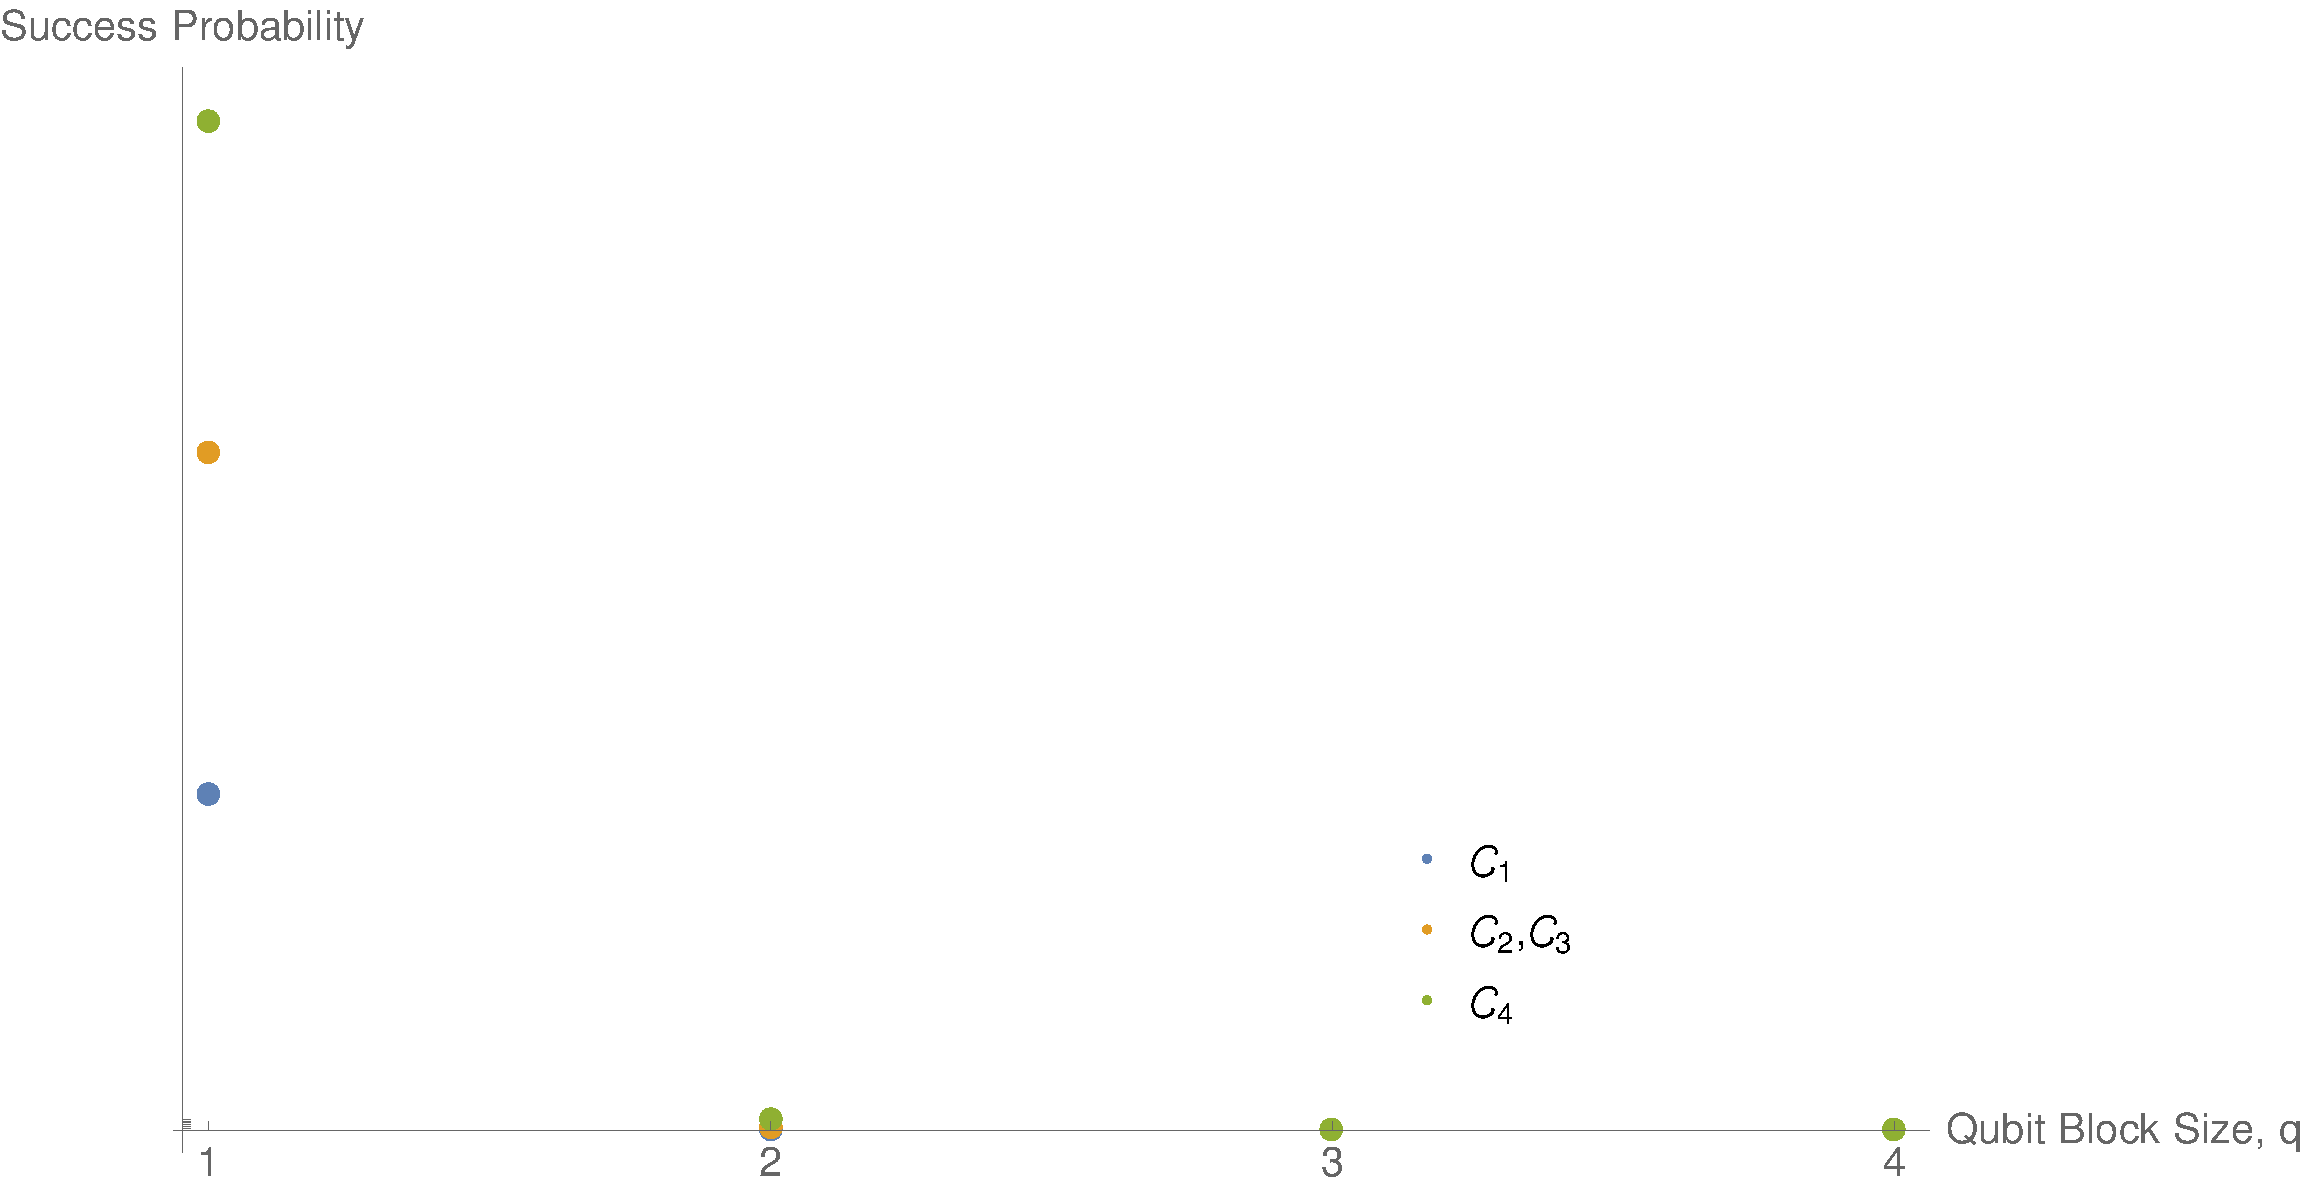
\includegraphics[width=0.5 \textwidth]{./blockencodingresults.pdf}
 	\caption{Maximum Observed Success probabilities for implementing a full $\mbox{CNOT}_{first,last}$ gate composed entirely of the sub-operations described in Tables~\ref{One Control Two Targets}-\ref{Four Controls two Targets}, for block size $q$.}
 	\label{Figure - Block Encoding Results}
 \end{figure}
 We immediately observe an order of magnitude increase in success probability of applying the $\mbox{CNOT}_{first,last}$ gate as we increase the size of our sub-operation components; refer to Fig.~\ref{Figure - Block Encoding Results}. This is a promising trend for applying entangling operations between blocks of qubits of size $q=3,4$ etc. Even within the reach of our numerical simulations, we find an improvement over standard KLM for applying entangling operations within the context of some quantum algorithms. For example, we can look at the toy quantum circuit 
 \begin{eqnarray}
 \small & \mbox{CNOT}^3 = \\ \small \nonumber & (I \otimes I \otimes \mbox{CNOT}) \cdot (I \otimes  \mbox{CNOT} \otimes I) \cdot (\mbox{CNOT} \otimes I \otimes I)
 \end{eqnarray}
 acting on four qubits presented in Fig.~\ref{Three CNOTs}. Through the standard KLM protocol acting on qubits encoded in the dual-rail, each CNOT gate can be implemented with success probabilty $2/27$ using ancilla resources $N_a,M_a=2$. Thus, we find the total cost of the $\mbox{CNOT}^3$ gate; a success probability of $(2/27)^3$ using ancilla resources $ N_a,M_a = 6 $. Grouping these four qubits into two deterministic blocks of two qubits, $q=2$ we can apply the same operation with a success probability of $0.00232161$ using ancilla resources $ N_a,M_a=4 $. This is almost a six-fold improvement, while using less ancillas.
 \begin{figure}[ht]
 	\centering
 	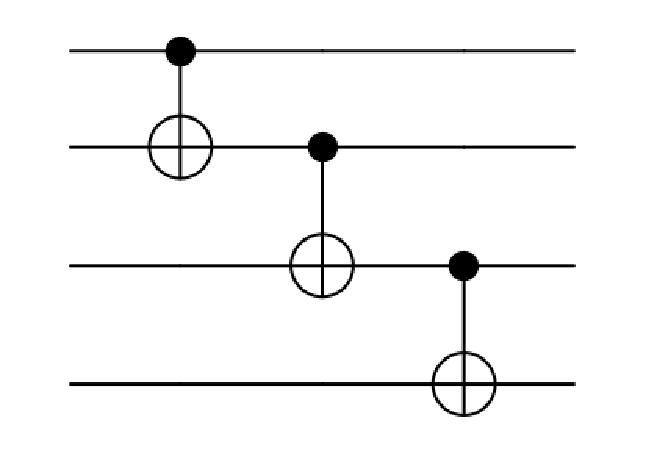
\includegraphics[width=0.25 \textwidth]{./ThreeCNOTs.pdf}
 	\caption{The general quantum circuit for the operator $\mbox{CNOT}^3$. The lines here represent logical qubits, not optical modes.}
 	\label{Three CNOTs}
 \end{figure}
\section{Conclusion}
\label{Section Conclusion}
 The trend in Fig.~\ref{Figure - Block Encoding Results} seems to suggest an order of magnitude improvement if we were able to simulate larger entangling operations between blocks. A realizable protocol for implementing $\mbox{CNOT}_{first,last}$ for $q \ge 3$ could have significant implications for LOQC.
\acknowledgments
Nicholas G. Sparks, Joshwa Shipman and Er. Knutson. This research was supported in part using high performance computing (HPC) resources and services provided by Technology Services at Tulane University, New Orleans, LA.
\appendix
\section{Proof of \textit{Fact 1}}
\label{Proof of Fact 1}
\textit{Fact 1} can be proved by induction. The base case is trivial; for a lone unitary matrix $U_1$,~(\ref{Fact 1}) reads
\begin{equation}
	A(U_1) = A(U_1)
\end{equation}
We can then assume
\begin{equation}
\label{Inductive Step}
	A(U_{P-1}) A(U_{P-2}) \dots A(U_1) = A(U_1 U_2 \dots U_{P-1})
\end{equation}
That is, applying the left hand side of~(\ref{Inductive Step}) is equivalent to the total transformation
\begin{equation}
	\hat{a}^\dagger_\alpha \rightarrow \sum_\beta (U_1 U_2 \dots U_{P-1})_{\alpha,\beta} \enspace \hat{a}^\dagger_\beta
\end{equation}
Now we add one final optical component and apply the transformation $A(U_P)$. Our total transformation is now
\begin{equation}
	\hat{a}^\dagger_\alpha \rightarrow \sum_\beta (U_1 U_2 \dots U_{P-1})_{\alpha,\beta} \Big(\sum_\gamma U_{\beta,\gamma}^P \hat{a}^\dagger_\gamma \Big)
\end{equation}
where $U_{\beta,\gamma}^P$ are the $\beta,\gamma$ elements of $U_P$. Then,
\begin{eqnarray}
\hat{a}^\dagger_\alpha \rightarrow \sum_{\beta,\gamma} (U_1 U_2 \dots U_{P-1})_{\alpha,\beta} U^P_{\beta,\gamma} \hat{a}^\dagger_\gamma
\\*
\hat{a}^\dagger_\alpha \rightarrow \sum_\gamma (U_1 U_2 \dots U_P)_{\alpha,\gamma} \hat{a}^\dagger_\gamma \quad
\end{eqnarray}
which is equivalent to $A(U_1 U_2 \dots U_n). \quad \quad\blacksquare $
\section{Proof of \textit{Fact 2}}
\label{Proof of Fact 2}
We can write~(\ref{LO State Fock Vec Basis}) in the $\ket{\vec{m}(\vec{n})}$ basis;
\begin{equation}
\ket{\psi} = \sum_{\vec{n}} c_{\vec{n}} \ket{\vec{m}(\vec{n})}
\end{equation}
We note that because photons are Bosons, and are indistinguishable, this change of basis is not well-defined. The same Fock state $\ket{\vec{n}}$ can map to multiple $\ket{\vec{m}(\vec{n})}$ states. This mapping is injective, however. No matter which mapping we choose for each basis state, no information about the state $\ket{\psi}$ is lost. Thus, we are free to pick any mapping we want for each basis Fock state. Then
\begin{equation}
\ket{\psi} = \sum_{\vec{n}} \frac{\vec{c}_n}{\prod_{p=1}^{M} \sqrt{n_p !}} \hat{a}_{m_1}^\dagger \hat{a}_{m_2}^\dagger \dots \hat{a}_{m_N}^\dagger \ket{\vec{0}}
\end{equation}
We define the vectors
\begin{equation}
\vec{U}_\alpha = (U_{\alpha 1},U_{\alpha 2},\dots U_{\alpha M})
\end{equation}
in the basis
\begin{equation}
\{ \hat{a}_{1}^\dagger,\hat{a}_{2}^\dagger, \dots, \hat{a}_{M}^\dagger \}
\end{equation}
then
\begin{eqnarray}
\label{Fact 2 Proof Checkpoint}
& \ket{\psi^\prime} = A(U) \ket{\psi} =  \quad \quad \quad \quad \quad \quad \quad \quad \quad \quad \\ & \nonumber
\sum_{\vec{n}} \frac{c_{\vec{n}}}{\prod_{p=1}^{M} \sqrt{n_p !}} \enspace \vec{U}_{m_1} \otimes \vec{U}_{m_2} \otimes \dots \otimes \vec{U}_{m_N} \ket{\vec{0}}
\end{eqnarray}
The tensor product in~(\ref{Fact 2 Proof Checkpoint}) will return a massive vector of $M^N$ entries. We can use the commutative property of the creation operators to compress it;
\begin{equation}
[\hat{a}_i ^ \dagger,\hat{a}_j ^ \dagger] = 0 \quad \forall \quad i,j
\end{equation}
\begin{eqnarray}
 \ket{\psi^\prime} = \sum_{\vec{n}} \frac{c_{\vec{n}}}{\prod_{p=1}^{M} \sqrt{n_p !}} \cdot \quad \quad \quad \quad \quad \quad \quad \quad \quad \\  \nonumber \sum^M_{\substack{m_1^\prime = 1\\
		m_2^\prime = m_1^\prime\\
		\vdots \\
		m_N^\prime = m_{N-1}^\prime}}
\left[ \sum_{perm(\vec{m}^\prime)} U_{m_1 m_1^\prime} \dots U_{m_N m_N^\prime} \right] \hat{a}_{m_1^\prime}^\dagger \dots \hat{a}_{m_N^\prime}^\dagger \ket{\vec{0}}
\end{eqnarray}
Finally, we define $\ket{\vec{n}^\prime(\vec{m}^\prime)}$ as the photo-counting result of $\hat{a}_{m_1^\prime}^\dagger \dots \hat{a}_{m_N^\prime}^\dagger \ket{\vec{0}}$, or the Fock state mapped to by each term in the summation over elements of $\ket{\vec{m}^\prime}$
\begin{eqnarray}
\label{Fact 2 Proof Checkpoint 2}
\small \ket{\psi^\prime} = \sum_{\vec{n}} c_{\vec{n}}  \cdot \quad \quad \quad \quad \quad \quad \quad \quad \quad \quad \quad \quad \quad \quad \quad \quad  \\ \sum^M_{\substack{m_1^\prime = 1\\
		m_2^\prime = m_1^\prime\\
		\vdots \\
		m_N^\prime = m_{N-1}^\prime}}
\left[ \prod_{p=1}^{M} \frac{\sqrt{n_p^\prime(\vec{m}^\prime) !}}{ \sqrt{n_p !}} \right] \left[ \sum_{perm(\vec{m}^\prime)} U_{m_1 m_1^\prime} \dots U_{m_N m_N^\prime} \right] \nonumber \\
\cdot \ket{\vec{n}^\prime (\vec{m}^\prime) } \quad \quad \quad \quad \quad \quad \quad \quad \quad \quad \quad \quad \quad \quad \quad \quad \nonumber
\end{eqnarray}
We recognize~(\ref{Fact 2 Proof Checkpoint 2}) as the result of a matrix vector product~(\ref{Matrix Vector Product}) if we define $A(U)$ as in~(\ref{Fact 2}).  $ \blacksquare $
\section{Proof of Facts 3 \& 4}
These are obvious statements that immediately follow from Eq.~(\ref{Matrix Vector Product})

\begin{thebibliography}{99}

\bibitem{KLM}  E. Knill, R. Laflamme, G. J. Milburn, Nature (London) 409, 46 (2001).

\bibitem{Uskov} Uskov Et. Al.
Phys. Rev. A 79, 042326 (2009).

\bibitem{Adami} https://arxiv.org/abs/quant-ph/9806048

\bibitem{Review Paper} Kok Et. Al.
Rev. Mod. Phys. 79, 135 (2007).

\bibitem{EIGEN} http://eigen.tuxfamily.org/

\end{thebibliography}


\end{document}
